\documentclass[letterpaper]{article}
\usepackage[utf8]{inputenc}
\usepackage[spanish,es-lcroman]{babel}
\usepackage{fancyhdr}
\usepackage{lastpage}
\usepackage{extramarks}
\usepackage[usenames,dvipsnames]{xcolor}
\usepackage{graphicx}
\usepackage{listings}
\usepackage{xparse}
\usepackage{courier}
\usepackage{float}
\usepackage{amsmath}
\usepackage{hyperref}
\usepackage{booktabs}


% Margenes
\topmargin=-0.45in
\evensidemargin=0in
\oddsidemargin=0in
\textwidth=6.5in
\textheight=9.0in
\headsep=0.25in


% Header y footer
\pagestyle{fancy}
\lhead{}
\chead{\guiaRamo\: \guiaTitulo} % Centro
\rhead{2015.2}
\lfoot{UTFSM-CSJ}
\cfoot{}
\rfoot{Página\ \thepage\ de\ \protect\pageref{LastPage}} % Pagina
\renewcommand\headrulewidth{0.4pt}
\renewcommand\footrulewidth{0.4pt}

\makeatletter
\newcommand{\titulo}[2]{%
  \vspace{#2}\noindent{#1}\vspace{\baselineskip}%
  \@afterindentfalse\@afterheading}
\makeatother


%------------------------------------------------------------------------
%	Meta Información
%------------------------------------------------------------------------
\newcommand{\guiaTitulo}{Tarea 2-3} % titulo del informe
\newcommand{\guiaFecha}{\today} % Fecha
\newcommand{\guiaRamo}{Seminario de Modelos y Métodos Cuantitativos} % Ramo
\newcommand{\guiaIniciales}{AL,JPEG} % Ramo
\newcommand{\guiaProfesor}{Andrés Moreira} % Profesor

%------------------------------------------------------------------------
%	Título
%------------------------------------------------------------------------
\title{
    \textmd{\textbf{\guiaRamo\\ \guiaTitulo}}\\
    \vspace{0.1in}
    \large{\textsc{Universidad Técnica Federico Santa María - Campus San Joaquín}}\\
    \normalsize\vspace{0.1in}\small{\guiaFecha}\\
    \vspace{0.1in}\large{\textit{Profesor \guiaProfesor}}
}
\author{
    \textsc{Juan Pablo Escalona G.} \\
    \small{juan.escalonag@alumnos.usm.cl} \\
    {\small 201073515-k}
    \and
     \textsc{Alonso Lepe M.} \\
    \small{alonso.lepe@alumnos.usm.cl}\\
    {\small 201173593-5}
\vspace{.5in}
}
\date{}

\begin{document}

\maketitle
\section{Pregunta 1}
Se tiene un grafo $G(n=400,p=1)$ esto implica que hay 79800 aristas que conectan a los 400 nodos entre todos. i.e. $\frac{399 \cdot 400}{2} = 79800$

Para que una componente conexa sea gigante debe tener un $k = np > 1$, en este caso $k = 400$, como se necesita un $k <= 1$ para que deje de ser gigante, entonces $p$ debería ser a lo mas $\frac{1}{400} = 0.0025$

Si se elimina una arista en el segundo 00:00:01 entonces aún quedan 79799 aristas, es decir, una probabilidad de $p = \frac{79799}{79800} = 0.9999$. Pero se sabe que se necesita una probabilidad de 0.0025, por lo que la componente dejará de ser conexa cuando solo hayan $\frac{E}{79800} = 0.0025 \implies E \sim 200$ aristas.

Luego si cada segundo se elimina 1 arista y es preciso eliminar 79600 aristas entonces se tendría que esperar hasta las 22:06:40 (10 de la noche, 6 minutos y 40 segundos)

\section{Pregunta 2}
La Matriz laplaciana de un grafo se puede obtener a partir de la matriz de adyacencia siguiendo el siguiente formato:
\begin{align}
  l_{i,j} =
  \begin{cases}
    k_i  & \text{si } i = j  \\
    -1  & \text{si } i \neq j  \\
    0  & \text{e.t.o.c.}
  \end{cases}
\end{align}
que es lo mismo que decir $l = K - A$ donde K es la matriz diagonal de los grados de cada nodo y A es la matriz de adyacencia. Luego para la matriz de adyacencia dada se tiene la siguiente matriz laplaciana:
\begin{align}
l = \begin{bmatrix}
   2  &-1  &-1  & 0  & 0  & 0    \\
   -1 &  2 & -1 &  0 &  0 &  0   \\
   -1 & -1 &  3 & -1 &  0 &  0   \\
    0 &  0 & -1 &  3 & -1 & -1   \\
    0 &  0 &  0 & -1 &  2 & -1   \\
    0 &  0 &  0 & -1 & -1 &  2
\end{bmatrix}
\end{align}

Luego el valor de Fielder es el segundo valor propio mas pequeño, en este caso corresponde a 0.438 ubicado en la tercera columna como se muestra en las ecuaciones (\ref{eq:fielder1}) y (\ref{eq:fielder2}).


\begin{align}
  V &= \begin{bmatrix}
     0.185 & -0.408 & \textbf{ 0.465} &  0.378 & -0.756 &  0.040 \\
     0.185 & -0.408 & \textbf{ 0.465} & -0.734 &  0.463 &  0.238 \\
    -0.657 & -0.408 & \textbf{ 0.261} &  0.357 &  0.292 & -0.278 \\
     0.657 & -0.408 & \textbf{-0.261} &  0.357 &  0.292 & -0.278 \\
    -0.185 & -0.408 & \textbf{-0.465} & -0.189 & -0.148 & -0.472 \\
    -0.185 & -0.408 & \textbf{-0.465} & -0.168 & -0.145 &  0.751
  \end{bmatrix} \label{eq:fielder1}\\
  E &= \begin{bmatrix} \quad 4.562 & \quad 0.000 & \; \textbf{0.438} & \quad 3.000 & \; \; 3.000 & \;\;\; 3.000 \end{bmatrix} \label{eq:fielder2}
\end{align}

Es importante ordenarlos para obtener el valor de Fielder, pues este es el segundo menor valor propio.
\begin{align}
  \text{Valor de Fielder: }  & \; 0.4384\\
  \text{Vector de Fielder: } & \begin{bmatrix}0.465 & 0.465 & 0.261 & -0.261 & -0.465 & -0.465\end{bmatrix}
\end{align}


\begin{figure}[H]
  \centering
  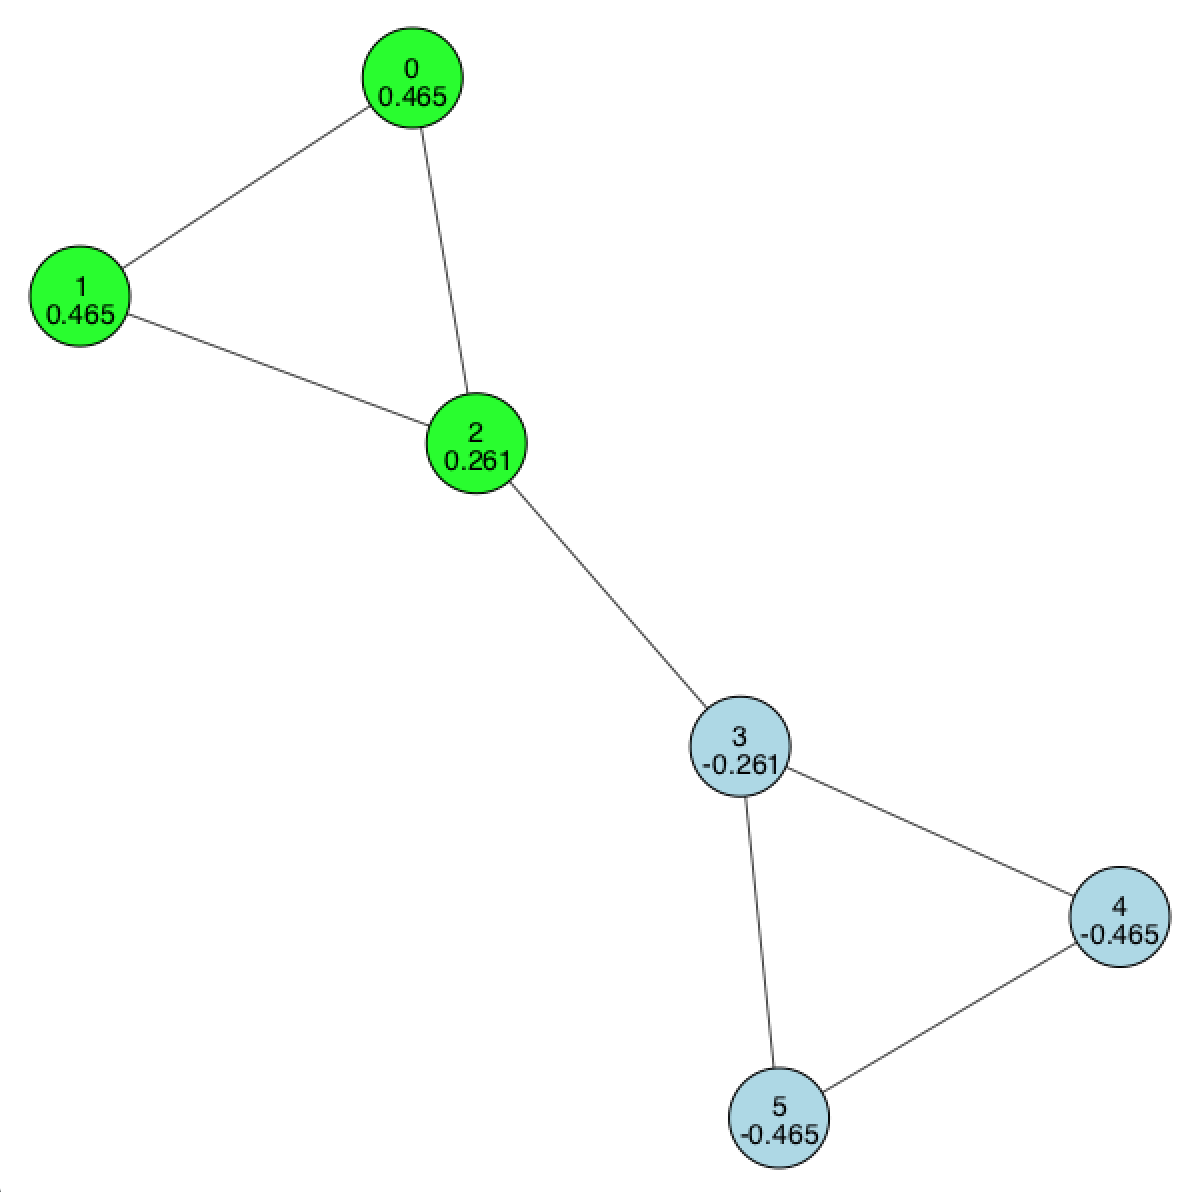
\includegraphics[width=.7\linewidth]{img/p2.png}
  \caption{Partición de la red en dos comunidades mostrando sus respectivos valores del vector propio.}
  \label{red:2}
\end{figure}

Se decidió cortar en el 0, pues los valores se separan uniformemente en torno al este. Se observan claramente dos comunidades en esta red las que interactúan únicamente por el vértice 2-3.


\section{Pregunta 4}

\subsection{Grafico de la red}
\begin{figure}[H]
  \centering
  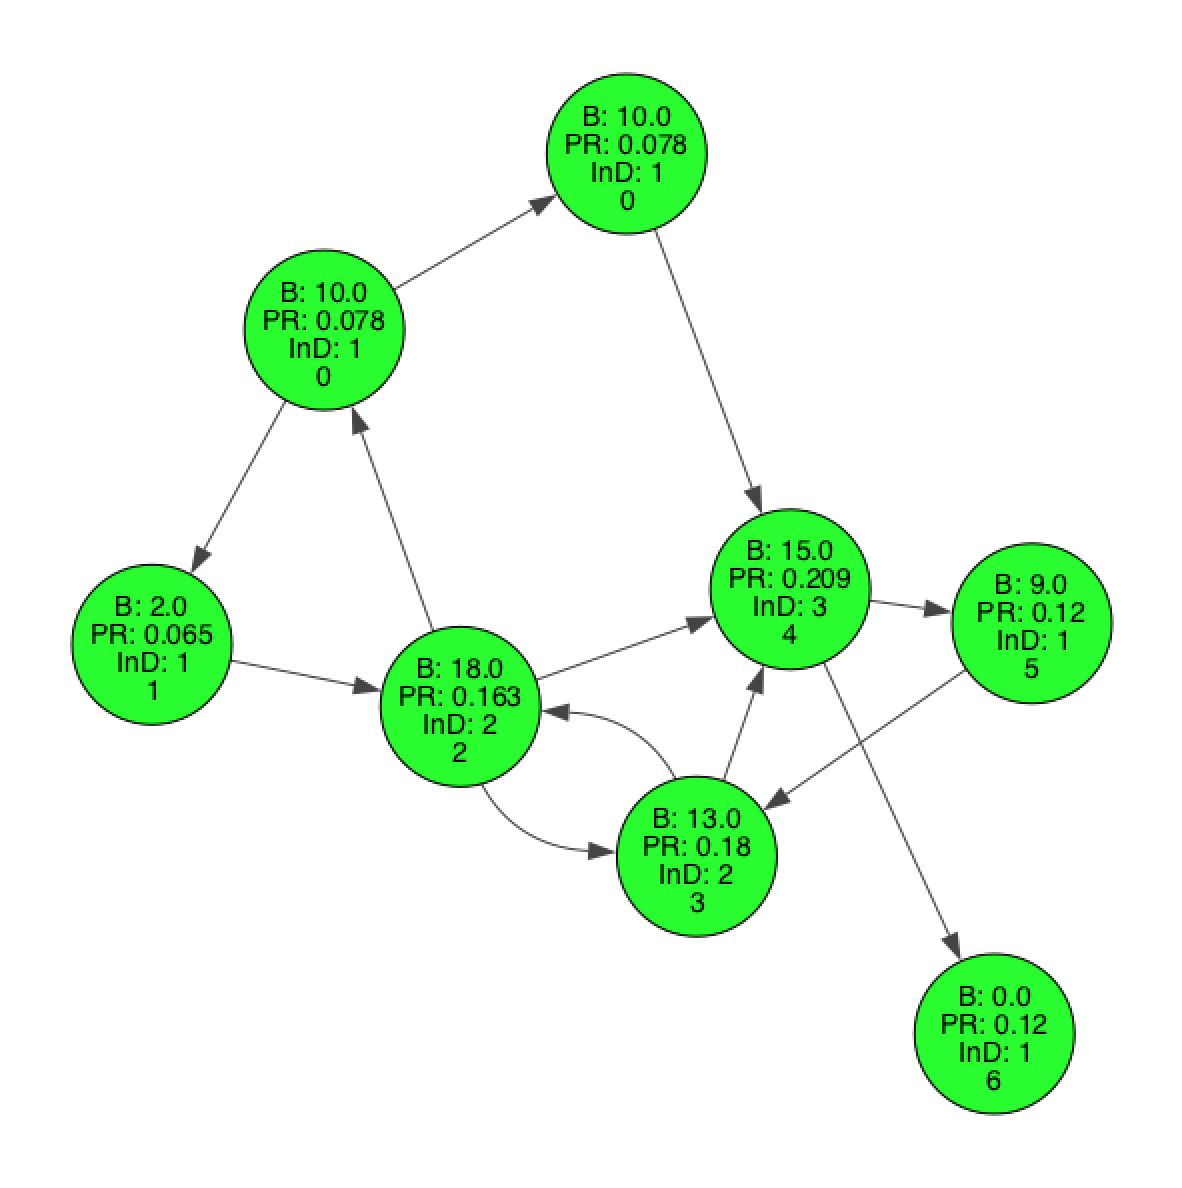
\includegraphics[width=.5\linewidth]{img/p4.png}
  \caption{Red chica dirigida. B: Betweenness, PR: PageRank, InD: Grado de entrada.}
  \label{red:4}
\end{figure}

\subsection{Ranking de los índices}
\begin{table}[H]
  \centering
  \renewcommand{\arraystretch}{1.1}
  \begin{tabular}{@{}ccccccccccc@{}}
    \toprule
       \multicolumn{3}{c}{\textsc{Grado Entrada}} & \phantom{abc} & \multicolumn{3}{c}{\textsc{Betweenness}} & \phantom{abc} & \multicolumn{3}{c}{\textsc{PageRank}}\\
       \cmidrule{1-3}\cmidrule{5-7}\cmidrule{9-11}
       Posición & Nodo & Valor & & Posición & Nodo & Valor & & Posición & Nodo & Valor\\
       \midrule
      1 & v5 & 3 &&  1 & v3 & 18 && 1 & v5 & 0.209 \\
      2 & v4 & 2 &&  2 & v5 & 15 && 2 & v4 & 0.180 \\
      2 & v3 & 2 &&  3 & v4 & 13 && 3 & v3 & 0.163 \\
      3 & v1 & 1 &&  4 & v1 & 10 && 4 & v6 & 0.120 \\
      3 & v2 & 1 &&  5 & v6 & 9  && 4 & v7 & 0.120 \\
      3 & v6 & 1 &&  6 & v8 & 3  && 5 & v1 & 0.078 \\
      3 & v7 & 1 &&  7 & v2 & 2  && 6 & v2 & 0.065 \\
      3 & v8 & 1 &&  8 & v7 & 0  && 6 & v8 & 0.065 \\
    \bottomrule
  \end{tabular}
  \caption{Ranking de cada índice para la red chica.}
\end{table}


\section{Referencias}
\section{Apéndice}

\end{document}
